\documentclass{beamer}
\usetheme{Antibes}
% \usecolortheme{seagull}
\useinnertheme{circles}
\usepackage{helvet}
\usepackage{graphicx}

\title{Beamer}
\subtitle{Introdução à Computação}
\author{Henrique Coelho}
\institute{Fundação Getúlio Vargas - EMAp}
% \institute{
\includegraphics[scale=0.4]{Imagens/EMAP.png}}
\date{19 de Abril de 2024}

\begin{document}
\begin{frame}[plain]
    \maketitle
\end{frame}
\section{Entrada Dramática}
\begin{frame}{Boing}
	\begin{block}{blocoinsano}
	Lorem ipsum dolor sit amet, consectetur adipiscing elit. Sed lacinia quis urna sit amet dapibus. Mauris efficitur justo nulla, quis eleifend erat malesuada ut. Vivamus blandit lacus a odio rutrum, non vestibulum mauris consectetur. Nam condimentum pretium luctus. Fusce ac tincidunt purus. Donec iaculis purus turpis. Praesent a placerat tortor. Donec at tempor elit, non consequat mi. Sed ornare dictum nulla. Integer luctus tortor diam, at blandit est dictum quis. Vestibulum sit amet nunc vestibulum, consectetur diam at, molestie neque. Nulla eros arcu, vestibulum id tincidunt vel, bibendum et lacus. Vivamus ac feugiat orci. Quisque ac vehicula odio, eu fringilla sem. Morbi sit amet ante vel diam faucibus maximus sit amet sed diam.
	\end{block}
\end{frame}
\section{A Grande Afirmação}
\begin{frame}{tartaruga legal}
	\begin{figure}[h!]
		\centering
		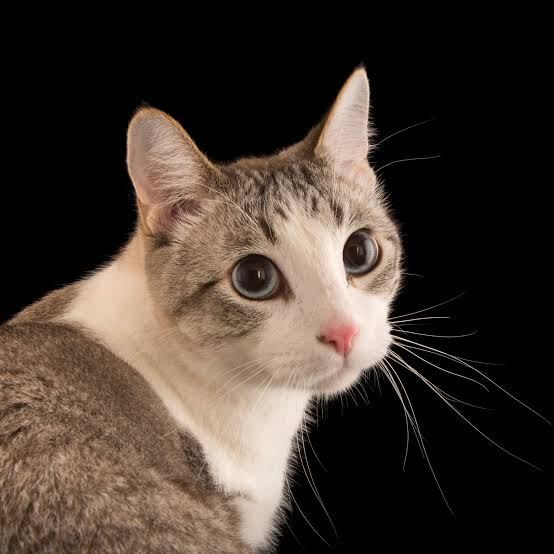
\includegraphics[width=0.5\linewidth]{Imagens/gato}
		\caption[Gato INSANO]{Talvez isso seja um cachorro.}
		\label{fig:gato}
	\end{figure}
\end{frame}

\section{Será?}
\begin{frame}{tartaruga?}
	\begin{block}{bloco INSANO da tartaruga:}
		\begin{itemize}
			\item legal
			\item chata
			\item tartaruga
		\end{itemize}
	\end{block}
	\begin{columns}
		\column{3cm}
		\begin{alertblock}{confusão}
			mano
		\end{alertblock}
		\column{6cm}
		\begin{exampleblock}{falácia}
		talvez isso não seja uma tartaruga
		\end{exampleblock}
	\end{columns}
\end{frame}

\end{document}
